\documentclass[unicode,12pt,aspectratio=169]{beamer}

\graphicspath{{../fig/}}
%%%%%%%%%%%%%%%%%%%%%%%%%%%
\usepackage{luatexja}% 日本語したい
\usepackage[haranoaji,no-math,deluxe,expert,nfssonly,match,scale=1.0]{luatexja-preset}
\renewcommand{\kanjifamilydefault}{\gtdefault}% 既定をゴシック体に

\usepackage{amssymb,amsmath,ascmac}

\usepackage{multirow}
\usepackage{lltjext}

\usepackage{siunitx}
\usepackage{physics}
\AtBeginDocument{\RenewCommandCopy\qty\SI}
\ExplSyntaxOn
\msg_redirect_name:nnn { siunitx } { physics-pkg } { none }
\ExplSyntaxOff

\usepackage{animate}
\usepackage{svg}
\usepackage{xparse}
%%%%%%%%%%%%%%%%%%%%%%%
\usepackage{tikz}
\usetikzlibrary{shapes,arrows}
\usetikzlibrary{positioning}
\usetikzlibrary{angles,quotes}
\usetikzlibrary{math, calc}
\usetikzlibrary{decorations.markings,decorations.pathmorphing}
%% define fancy arrow. \tikzfancyarrow[<option>]{<text>}. ex: \tikzfancyarrow[fill=red!5]{hoge}
\tikzset{arrowstyle/.style n args={2}{inner ysep=0.1ex, inner xsep=0.5em, minimum height=2em, draw=#2, fill=black!20, font=\sffamily\bfseries, single arrow, single arrow head extend=0.4em, #1,}}
\NewDocumentCommand{\tikzfancyarrow}{O{fill=black!20} O{none}  m}{
\tikz[baseline=-0.5ex]\node [arrowstyle={#1}{#2}] {#3 \mathstrut};}

%目次スライド
% \AtBeginSection[]{
%   \frame{\tableofcontents[currentsection]}
% }
%アペンディックスのページ番号除去
\newcommand{\backupbegin}{
\newcounter{framenumberappendix}
\setcounter{framenumberappendix}{\value{framenumber}}
}
\newcommand{\backupend}{
\addtocounter{framenumberappendix}{-\value{framenumber}}
\addtocounter{framenumber}{\value{framenumberappendix}} 
}

%%%%%%%%%%%  theme  %%%%%%%%%%%
% \usetheme{Copenhagen}
\usetheme{metropolis}
% \usetheme{CambridgeUS}
% \usetheme{Berlin}

%%%%%%%%%%%  inner theme  %%%%%%%%%%%
% \useinnertheme{default}

% %%%%%%%%%%%  outer theme  %%%%%%%%%%%
\useoutertheme{default}
% \useoutertheme{infolines}

%%%%%%%%%%%  color theme  %%%%%%%%%%%
%\usecolortheme{structure}

%%%%%%%%%%%  font theme  %%%%%%%%%%%
\usefonttheme{professionalfonts}
%\usefonttheme{default}

%%%%%%%%%%%  degree of transparency  %%%%%%%%%%%
%\setbeamercovered{transparent=30}

%%%%%%%%%%%  numbering  %%%%%%%%%%%
% \setbeamertemplate{numbered}
\setbeamertemplate{navigation symbols}{}
\setbeamertemplate{footline}[frame number]

%%%%%%%%%%%%%%%%%%%%%%%%%%%%%%%%%%%
% \setbeamertemplate{items}[default]
\setbeamertemplate{enumerate item}[default]

% セクション名だけをTOCに出力
\setcounter{tocdepth}{1}



\title{第四章 線形動的粘弾性について}
\date{\empty}

\begin{document}

\section{動的な刺激への応答}
\subsection{動的刺激としての波}

\begin{frame}
	\frametitle{動的な刺激としての波}

	\begin{itemize}
		\item 物理的実験では、動的な刺激として波を用いる
		\item 振幅および周期が一定の波としてサインカーブを用いる場合が多い
		\item<2-> 時間変化するサイン波のイメージを示した
	\end{itemize}
	\vspace{2mm}
		\centering
		\only<1>{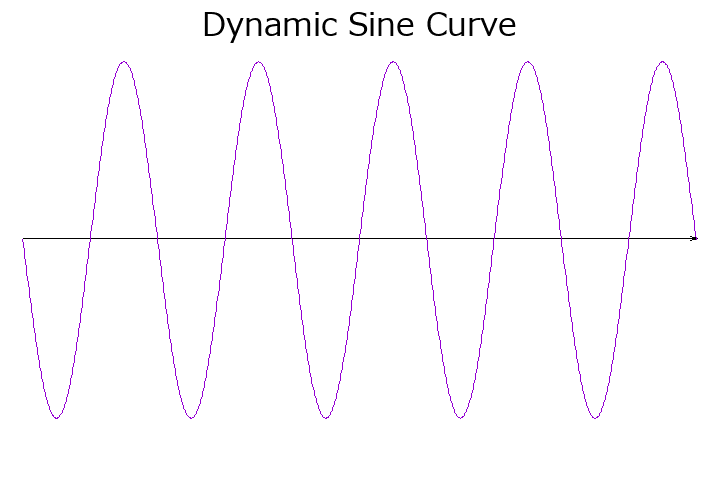
\includegraphics[width=0.5\textwidth]{sin_curve/image_001}}
		\only<2>{\animategraphics[loop, width=0.5\textwidth, autoplay]{10}{sin_curve/image_}{001}{051}}
\end{frame}


\begin{frame}
	\frametitle{動的な刺激について}
	\begin{block}{動的なひずみとは？}
		\begin{itemize}
			\item 周期（繰り返し）的に時間変化するひずみ $\gamma (t)$
			\item $\omega t = 2\pi$で一周期（円を一周）となる
		\end{itemize}
		\begin{equation*}
			\gamma (t) = \gamma_0 \sin(\omega t)
		\end{equation*}
	\end{block}

	\begin{block}{$\omega$は角周波数で、回転速度を表すスカラー量}
		\begin{columns}[T, onlytextwidth]
			\column{.48\linewidth}
			\footnotesize

			\vspace{3mm}
			\begin{equation*}
				\omega \equiv \dfrac{\mathrm{d} \theta}{\mathrm{d} t} = \dfrac{2 \pi}{T} = 2\pi f
			\end{equation*}
			\vspace{-3mm}
			\begin{itemize}
				\item $\theta$：角度 (単位：ラジアン)
				\item $T$ ：周期 (単位：秒)
				\item $f$ ：周波数 (単位：ヘルツ)
			\end{itemize}
			\column{.48\linewidth}
			\footnotesize
			\begin{itemize}
				\item $\theta$ が無次元量なので$\omega$ の次元は $\mathrm{T}^{-1}$
				\item SI 単位では、ラジアン毎秒 (rad/s)
				\item 角周波数は通常の周波数を単純に\\$2\pi$ 倍したもの
			\end{itemize}
		\end{columns}
	\end{block}
\end{frame}

\begin{frame}{周期的な入力のイメージ}
	\begin{block}{等速円運動 $\Leftrightarrow$ 単振動 $\Leftrightarrow$ 波動は等価}
		$\sin(\omega t)$ 等の三角関数の組み合わせで記述できる。

		\vspace{1mm}
		\centering
		\animategraphics[loop, width=0.6\textwidth, autoplay]{20}{vibration/vibration-}{0}{50}
	\end{block}
\end{frame}


\end{document}